% subseccion 4.2
\subsection{Etapa 2: Búsqueda de Estudios}
Esta etapa presenta la estrategia de búsqueda usada en la revisión sistemática de la literatura. Esta estrategia se describe en detalle en las subsecciones~\ref{subsubsec:Definiendo la Estrategia de Busqueda} -- \ref{subsubsec:resultados-busqueda}. Ver figura~\ref{fig:etapa2}.

\begin{figure*}[tbp]
    \centering
    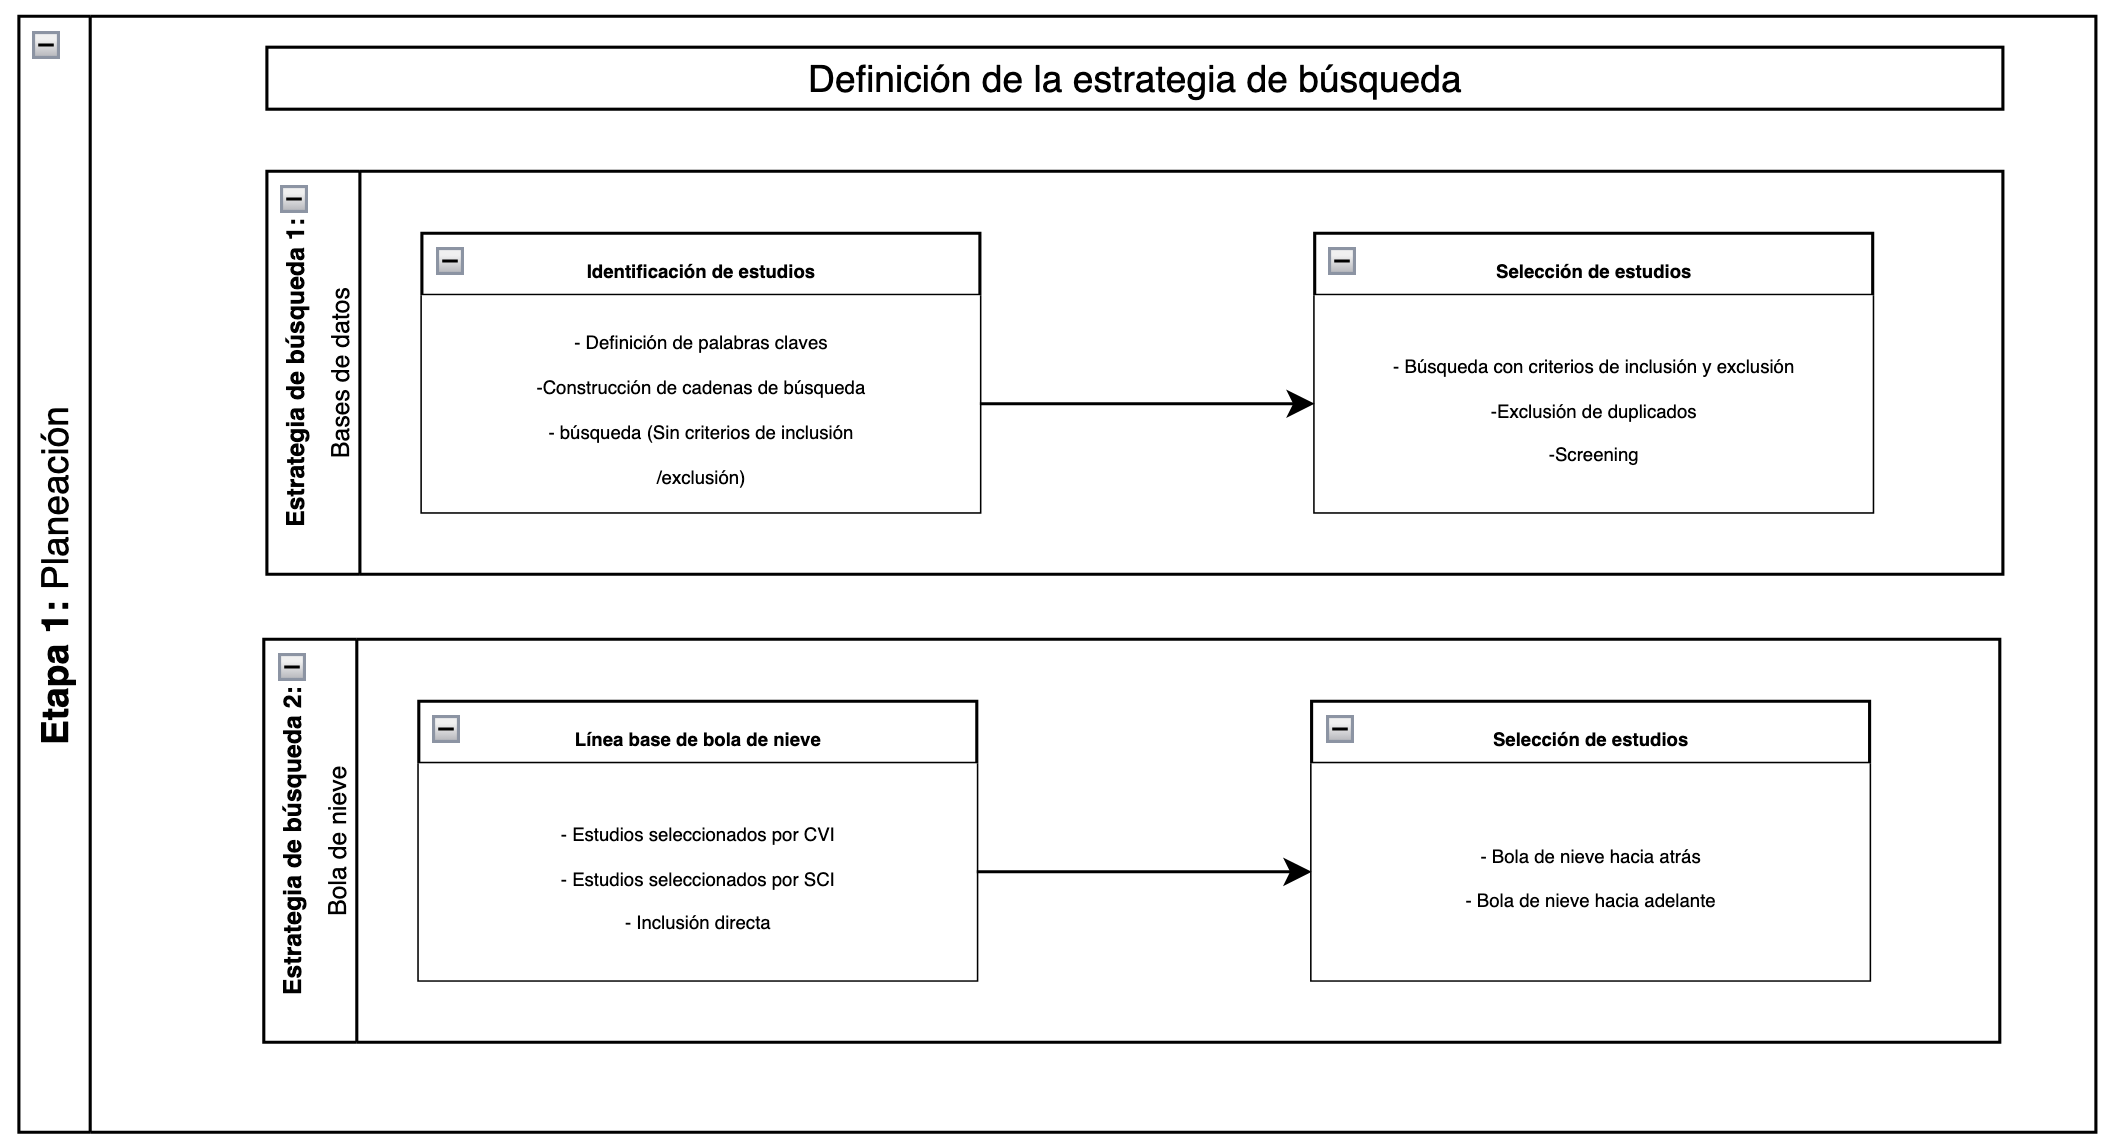
\includegraphics[width=0.8\textwidth]{resources/images/planeacion/estrategias-busqueda.png}
    \caption{Composición de la etapa de búsqueda de estudios}\label{fig:etapa2}
\end{figure*}

%sub-subseccion 4.2.1 
\subsubsection{Definiendo la Estrategia de Búsqueda}\label{subsubsec:Definiendo la Estrategia de Busqueda}
\mbox{}\\
% Content for 4.2.1
Para la construcción de esta revisión de la literatura, se usó un enfoque híbrido. Con este enfoque se busca obtener mayor volumen de artículos indexados y con diferentes origenes. más allá de los proporcionados por las bases de datos.
En este sentido, se combinaron dos estrategias de búsqueda. La primer estrategia es la búsqueda en bases de datos y consiste en realizar una cadena de búsqueda automatizada en bases de datos académicas.~\cite{jalali2012systematic}.
La segunda estrategia es la denominada ``Bola de Nieve'' (Snowballing) y consiste en la búsqueda manual de artículos a partir de un conjunto base de artículos usando las referencias y las citas de los mismos. Esta estrategia se basa en la premisa de que los artículos relevantes citan otros artículos relevantes y, por lo tanto, permite encontrar artículos que no están indexados en las bases de datos académicas.~\cite{jalali2012systematic} y \cite{goodman1961snowball}.
\mbox{}\\
%sub-subseccion 4.2.2
\subsubsection{Estrategia de Búsqueda 1: Bases de Datos}
\mbox{}\\
Esta estrategia consta de 2 componentes. El primer componente es denominado ``Identificación de estudios''. Esto se enfoca en definir las palabras clave para construir las cadenas de búsqueda que conducen a completar las búsquedas en las bases de datos académicas.
\mbox{}\\

% sub-subsetion for 4.2.3
\subsubsection{Estrategia de Búsqueda 2: Bola de Nieve (Snowballing)}
Quis ut deserunt in nulla aliquip exercitation. Voluptate non laborum do eu dolor mollit officia cupidatat do ea id id ullamco. Dolore velit anim est pariatur eiusmod occaecat duis labore reprehenderit nisi esse. Eu laboris cillum ullamco non velit veniam labore eiusmod laboris sint. Consequat officia aliquip velit officia do ex nulla cupidatat elit dolore deserunt sint.
\mbox{}\\

% sub=-subsection 4.2.4
\subsubsection{Resultados de la Búsqueda de Estudios}
\label{subsubsec:resultados-busqueda}
Nostrud enim magna culpa labore in culpa aliqua dolore ea amet sit magna exercitation sunt. Voluptate qui aliqua velit ipsum ullamco dolor ad velit cupidatat dolore sint. Nisi cillum dolore magna tempor minim ullamco anim quis ipsum consequat officia.
\mbox{}\\